\documentclass[12pt,a4paper]{article}
\usepackage[UTF8]{ctex}
\usepackage{amsmath}
\usepackage{graphicx}
\usepackage{booktabs}
\usepackage{geometry}
\usepackage{ulem}
\geometry{left=2.5cm,right=2.5cm,top=2.5cm,bottom=2.5cm}

\title{\Huge{\textbf{\uuline{实\ 验\ 报\ 告}}}}
\author{\uline{少年班学院} \quad 姓名: \uline{李大恕} \quad 学号: \uline{PB24000145} \quad 实验日期: \uline{2025--3--17}}
\date{\today}

\begin{document}

\maketitle

\section{实验题目}
	单摆法测重力加速度

\section{实验目的}
    \begin{enumerate}
        \item 掌握单摆测量重力加速度的原理和方法
        \item 学习基本长度测量仪器的使用
        \item 掌握实验数据处理和不确定度计算方法
    \end{enumerate}

\section{实验原理}
    根据单摆周期公式：
    \begin{equation}
        T = 2\pi \sqrt{\frac{L}{g}}
    \end{equation}
    可得重力加速度计算公式：
    \begin{equation}
        g = \frac{4\pi^2 L}{T^2}
    \end{equation}
    式中：
    \begin{itemize}
        \item $T$ —— 单摆周期（s）
        \item $L$ —— 摆长（m）
        \item $g$ —— 重力加速度（m/s²）
    \end{itemize}

\section{实验器材}
    \begin{itemize}
        \item 单摆装置
        \item 钢球（直径$d=2.00\ \mathrm{cm}$）
        \item 电子秒表（精度0.01s）
        \item 游标卡尺（精度0.02mm）
        \item 米尺（精度1mm）
    \end{itemize}

\section{基础内容}
    \subsection{实验步骤}
        \begin{enumerate}
            \item 测量摆长$L$：用米尺测量摆线长度$l$，用游标卡尺测量摆球直径$d$，则$L=l+d/2$
            \item 调整摆角小于5°
            \item 测量周期：记录单摆完成30次全振动的时间$t$，重复测量6次
            \item 计算重力加速度$g$
            \item 进行不确定度分析
        \end{enumerate}

    \subsection{数据处理}
        \subsubsection{原始数据记录}
            \begin{center}
                \begin{tabular}{ccccccc}
                    \toprule
                    次数 & 1 & 2 & 3 & 4 & 5 & 6 \\
                    \midrule
                    $L$ (cm) & 65.10 & 65.05 & 65.04 & 65.05 & 65.07 & 65.05 \\
                    $t$ (s) & 48.49 & 48.41 & 48.44 & 48.43 & 48.35 & 48.42 \\
                    \bottomrule
                \end{tabular} \\
                \textbf{表1：原始数据}
            \end{center}
           
        \subsubsection{数据处理计算}
            周期平均值：
            \[
                \overline{T}=\frac{1}{n}\sum_{i=1}^{n}T_i=\frac{1.6163+1.6137+1.6147+1.6143+1.6117+1.614}{6}\,\mathrm{s}=1.6141\,\mathrm{s}
            \]

            摆长平均值：
            \[
                \overline{L}=\frac{1}{n}\sum_{i=1}^{n}L_i=\frac{65.1+65.05+65.04+65.05+65.07+65.05}{6}\,\mathrm{cm}=65.06\,\mathrm{cm}=0.6506\,\mathrm{m}
            \]
            
            重力加速度计算：
            \[
                g=\frac{4 \pi^{2} L}{T^{2}}=\frac{4\times \pi^2\times 0.6506}{1.6141^2}\,\mathrm{m/s^2}=9.8584\,\mathrm{m/s^2}
            \]

        \subsubsection{不确定度分析}
            \begin{enumerate}
                \item 摆长$L$的不确定度： \\
                摆长$L$的标准差
                \[
                    \begin{aligned}
                        \sigma_{L}&=\sqrt{\frac{1}{n-1}\sum_{i=1}^n\left(l_i-\overline{l}\right)^2} \\
                        &=0.021909\,\mathrm{cm}
                    \end{aligned}
                \]
                摆长$L$的B类不确定度
                \[
                    \Delta_{B,L}=\sqrt{\Delta_\text{仪}^2+\Delta_\text{估}^2}=\sqrt{0.2^2+0.05^2}\,\mathrm{cm}=0.20616\,\mathrm{cm}
                \]
                摆长$L$的展伸不确定度
                \[
                    \begin{aligned}
                        U_{L,P}&=\sqrt{\left(t_P\frac{\sigma_{l}}{\sqrt{n}}\right)^2+\left(k_P\frac{\Delta_{B,L}}{C}\right)^2} \\
                        &=\sqrt{\left(2.57\times\frac{0.021909}{\sqrt{6}}\right)^2+\left(1.96\times\frac{0.20616}{3}\right)^2}\,\mathrm{cm} \\
                        &=0.13664\,\mathrm{cm},P=0.95
                    \end{aligned}
                \]

                \item 周期$T$的不确定度： \\
                周期$T$的标准差
                \[
                    \begin{aligned}
                        \sigma_{T}&=\sqrt{\frac{1}{n-1}\sum_{i=1}^n\left(T_i-\overline{T}\right)^2}\\
                        &=0.0015154\,\mathrm{s}
                    \end{aligned}
                \]
                周期$T$的B类不确定度
                \[
                    \Delta_{B,T}=\sqrt{\Delta_\text{仪}^2+\Delta_\text{估}^2}=\sqrt{0.00033333^2+0.0066667^2}\,\mathrm{s}=0.006675\,\mathrm{s}
                \]
                周期$T$的展伸不确定度
                \[
                    \begin{aligned}
                        U_{T,P}&=\sqrt{\left(t_P\frac{\sigma_{T}}{\sqrt{n}}\right)^2+\left(k_P\frac{\Delta_{B,T}}{C}\right)^2}\\
                        &=\sqrt{\left(2.57\times\frac{0.0015154}{\sqrt{6}}\right)^2+\left(1.96\times\frac{0.006675}{3}\right)^2}\,\mathrm{s}\\
                        &=4.6418 \times 10^{-3}\,\mathrm{s},P=0.95
                    \end{aligned}
                \]

                \item 重力加速度$g$的不确定度： \\
                重力加速度$g$的延伸不确定度
                \[
                    \begin{aligned}
                        U_{g,P}&=\sqrt{\left(\frac{\partial g}{\partial L}U_{L,P}\right)^2+\left(\frac{\partial g}{\partial T}U_{T,P}\right)^2}\\
                        &=\sqrt{\left(\frac{4 \pi^{2}}{T^{2}}U_{L,P}\right)^2+\left(- \frac{8 \pi^{2} L}{T^{3}}U_{T,P}\right)^2}\\
                        &=\sqrt{\left(\frac{4\times \pi^2}{1.6141^2}\times 0.0013664\right)^2+\left(-\frac{8\times \pi^2\times 0.6506}{1.6141^3}\times 0.0046418\right)^2}\,\mathrm{m/s^2}\\
                        &=0.060363\,\mathrm{m/s^2},P=0.95
                    \end{aligned}
                \]
                重力加速度$g$最终结果
                \[
                    g=\left(9.86 \pm 0.06\right)\,\mathrm{m/s^2}
                \]

            \end{enumerate}

    \section{提升内容}
        \subsection{实验步骤}
            \begin{enumerate}
                \item 测量摆长$L$：用米尺测量摆线长度$l$，用游标卡尺测量摆球直径$d$，则$L=l+d/2$
                \item 调整摆角小于5°
                \item 测量周期：记录单摆完成30次全振动的时间$t$，改变摆长$L$，测量6次
                \item 利用最小二乘法线性拟合$L$与$T^2$的关系，得出$g$的值
                \item 进行不确定度分析
            \end{enumerate}

        \subsection{数据处理}
            \subsubsection{原始数据记录}
                \begin{center}
                    \begin{tabular}{ccccccc}
                        \toprule
                        次数 & 1 & 2 & 3 & 4 & 5 & 6 \\
                        \midrule
                        $L$ (cm) & 54.33 & 57.17 & 59.98 & 65.42 & 69.37 & 72.55 \\
                        $t$ (s) & 44.17 & 45.31 & 46.63 & 48.72 & 49.98 & 51.23 \\
                        \bottomrule
                    \end{tabular} \\
                    \textbf{表2：原始数据}
                \end{center}

            \subsubsection{数据处理计算}
                采用最小二乘法线性拟合$L$与$T^2$的关系，得到线性方程：$L=mT^2+b$
                \begin{center}
                    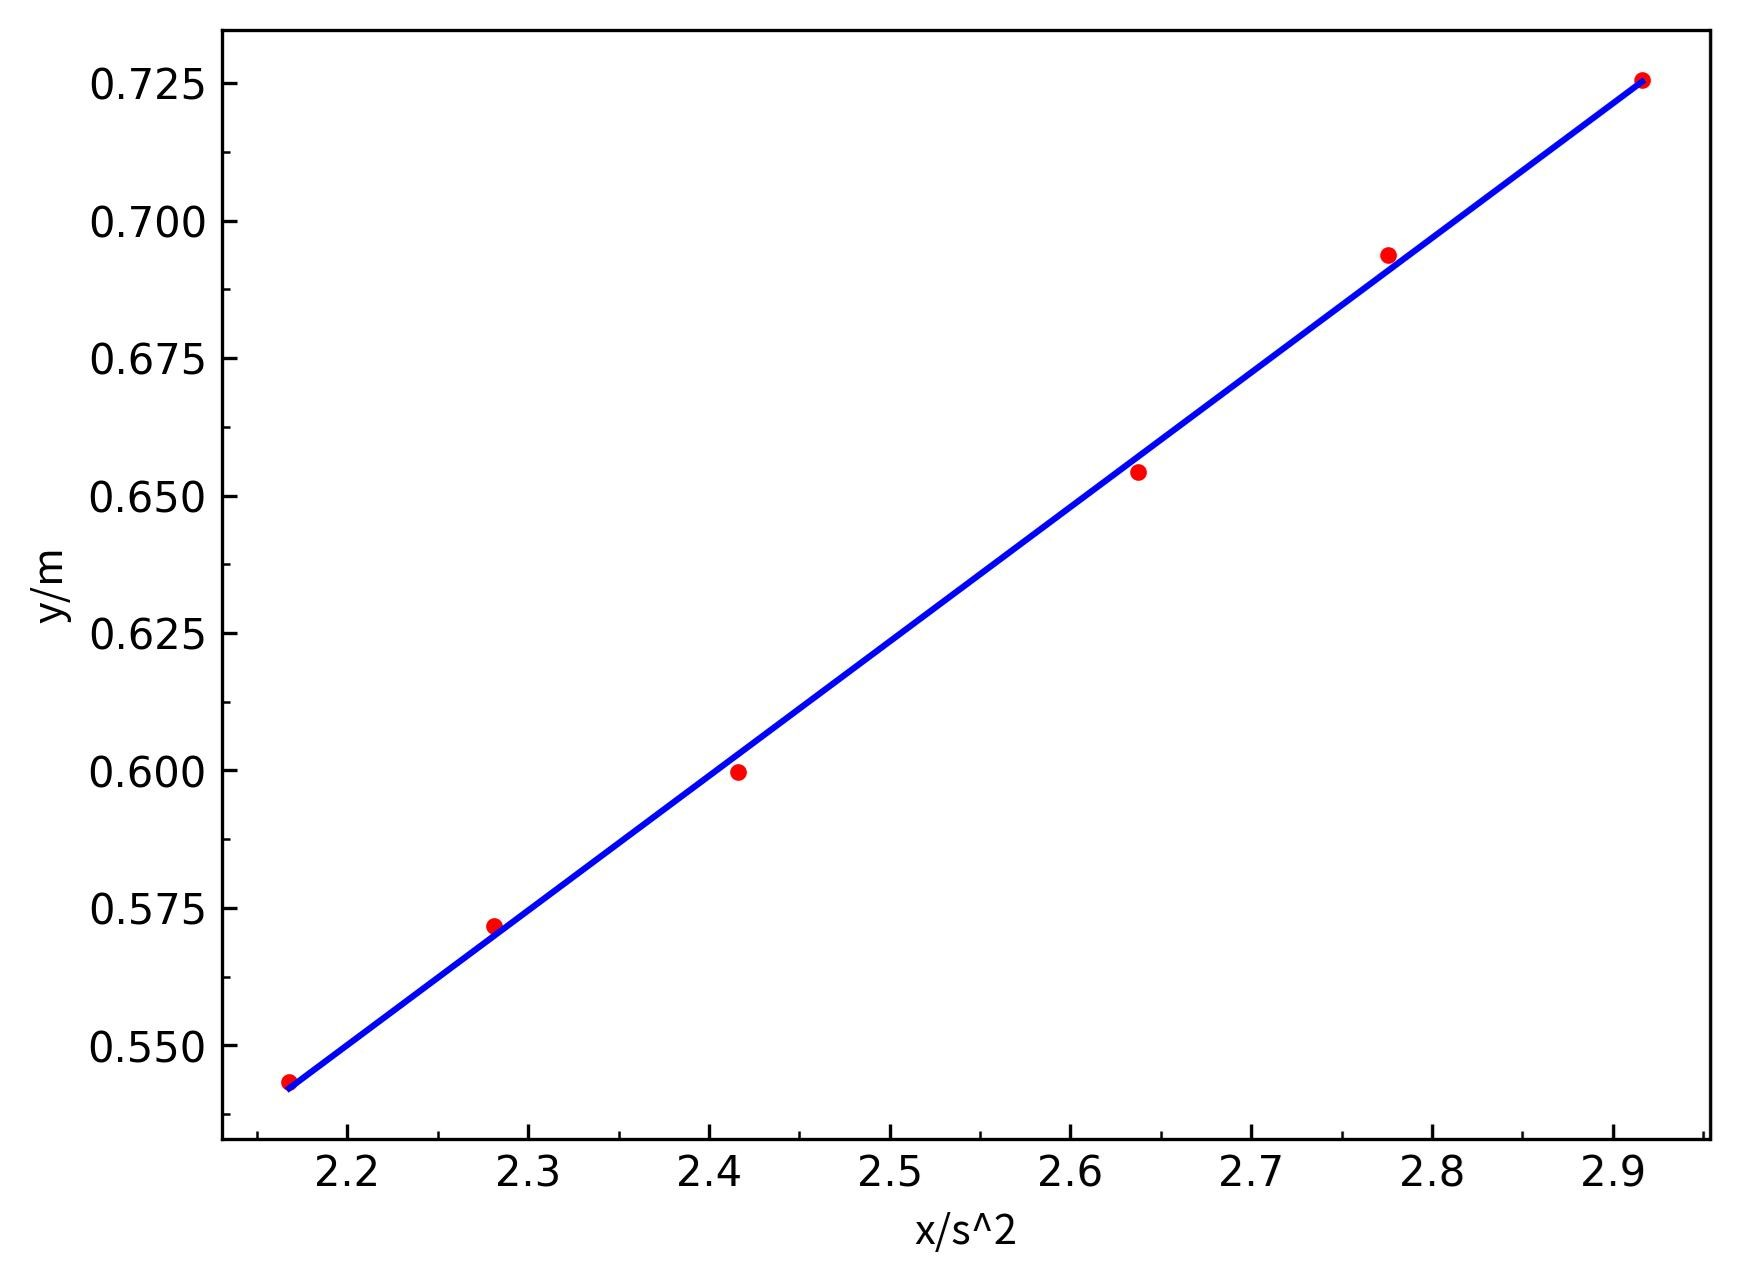
\includegraphics[width=0.8\textwidth]{最小二乘法.jpg} \\
                    \textbf{图1：最小二乘法线性拟合}
                \end{center}

                斜率
                \[
                    m=0.2446\,\mathrm{m/s^2}
                \]

                截距
                \[
                    b=0.01197\,\mathrm{m}
                \]

                线性拟合的相关系数
                \[
                    r=\frac{\overline{xy}-\overline{x}\cdot\overline{y}}{\sqrt{\left(\overline{x^2}-\overline{x}^2\right)\left(\overline{y^2}-\overline{y}^2\right)}}=0.99940694
                \]

                又$T=2\pi\sqrt{\frac{L}{g}}$，所以
                \[
                    L = \frac{g}{4\pi^2}T^2
                \]
                则
                \[
                    g = 4\pi^2m = 4\pi^2\times0.2446\,\mathrm{m/s^2} = 9.65\,\mathrm{m/s^2}
                \]

            \subsubsection{不确定度分析}
                斜率的不确定度
                \[
                    u_m=\lvert m\rvert\cdot\sqrt{\frac{1}{n-2}\left(\frac{1}{r^2}-1\right)}=0.004214\,\mathrm{m/s^2}
                \]
                则
                \[
                    u_g=4\pi^2u_m=0.166358\,\mathrm{m/s^2}
                \]
            
    \section{进阶内容}
        利用智能手机录制了一段帧率为60FPS的大角度单摆（摆角约为$10^\circ$）运动视频。用视频追踪技术（Tracker）获取单摆的运动轨迹，研究运动规律。Tracker从该视频中获取有效数据点3588个，对运动轨迹数据进行拟合分析。以下是运动轨迹拟合及x-t和y-t图象：\\
        \begin{center}
            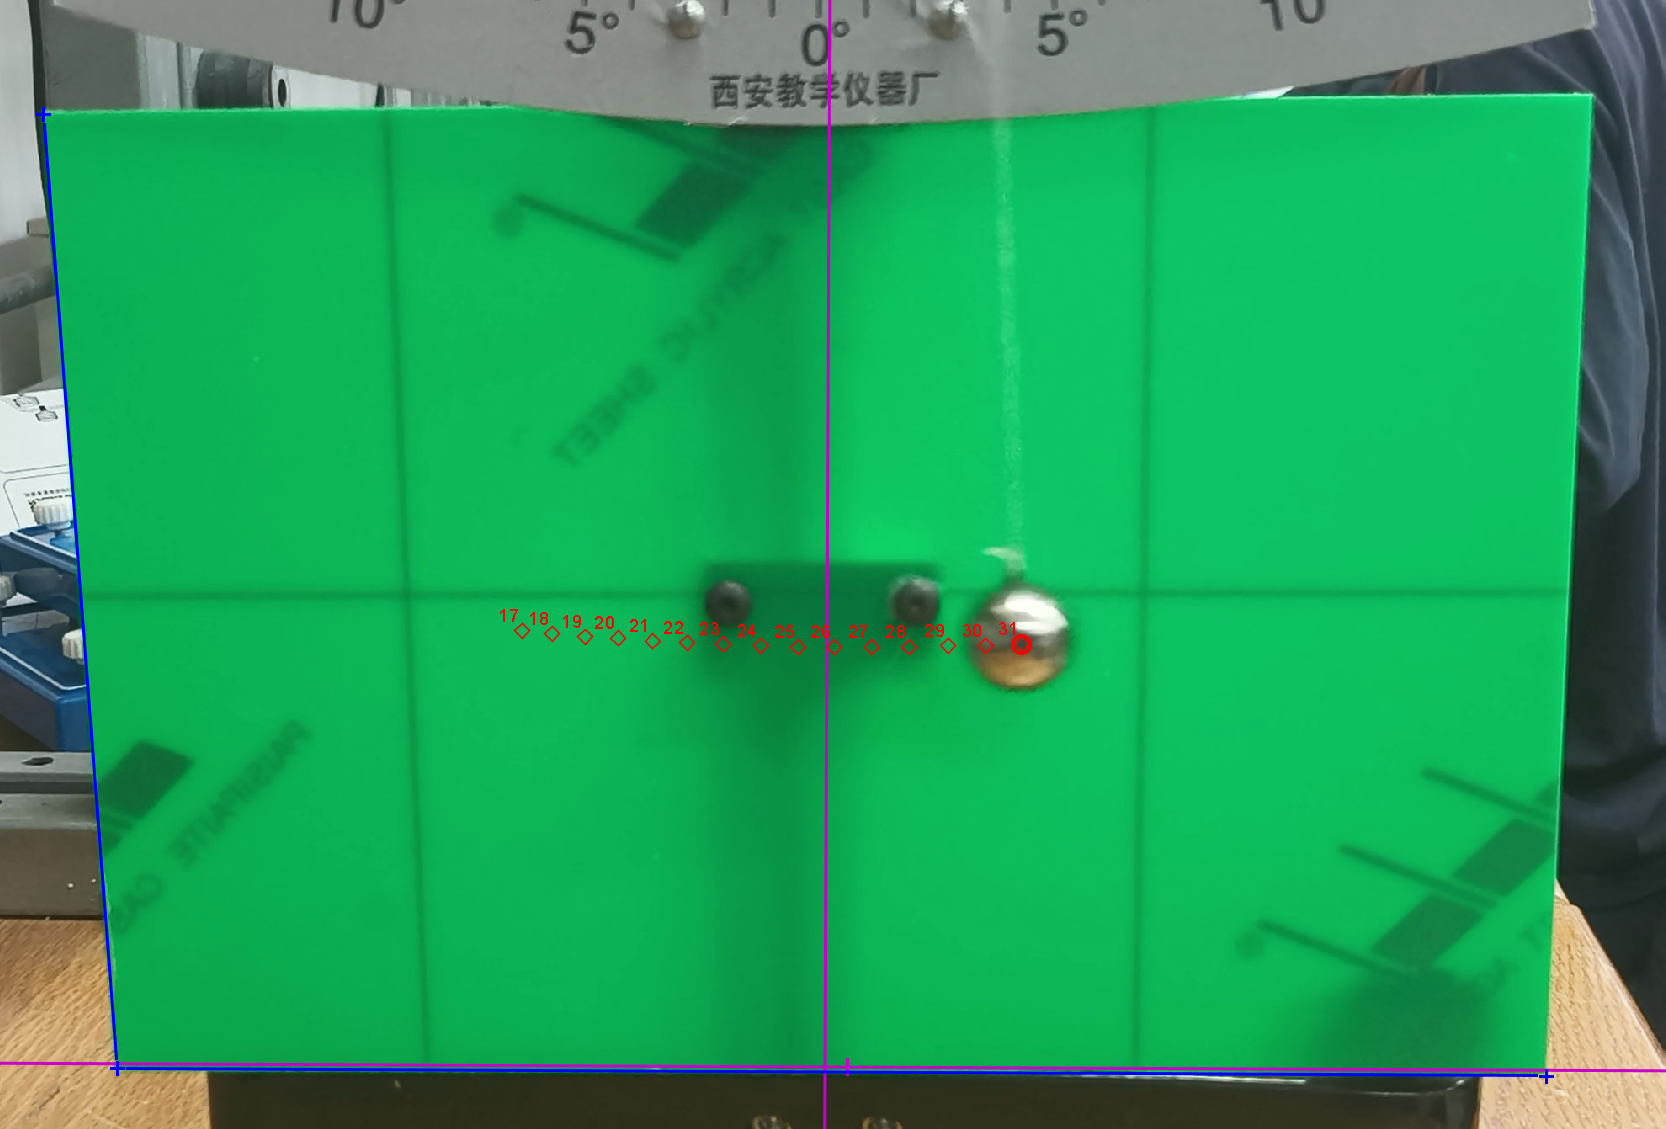
\includegraphics[width=0.8\textwidth]{Tracker-1.png} \\
            \textbf{图2：Tracker运动轨迹} \\
            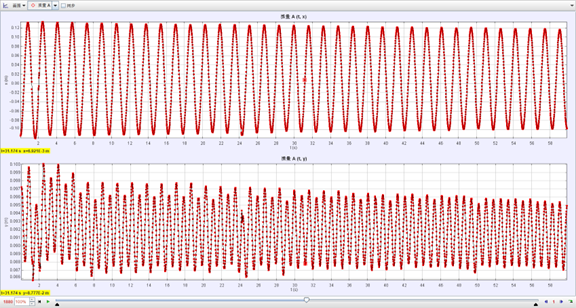
\includegraphics[width=0.8\textwidth]{Tracker-2.png} \\
            \textbf{图3：运动的x-t及y-t图像}
        \end{center}
        
        考虑到空气阻力的影响，单摆的运动可修正为阻尼振动，振动周期与阻尼系数有关。即$\omega'=\sqrt{\omega_0^2-\gamma^2}$，其中$\omega_0=\sqrt{g/L}$为单摆的固有频率，$\gamma$为阻尼系数。此时，振幅随时间变化，$A=A_0\mathrm{e}^{-\gamma t}$。 \\

        实验拍摄了较长时间的单摆摆动视频，利用Tracker软件分析了单摆的运动轨迹。通过对数据进行拟合，得到了$\gamma$和$\omega$的值：\\
        \[\gamma=(2.36\pm 0.02)\times 10^{-3}\,\mathrm{s^{-1}}\]
        \[\omega=(3.88525\pm 0.00002)\,\mathrm{s^{-1}}\]
        由此可以计算出单摆的固有频率$\omega_0$：
        \[
            \omega_0=\sqrt{\omega^2+\gamma^2}=(3.88525\pm 0.00002)\,\mathrm{s^{-1}}
        \]
        通过米尺测得摆长为$L=(0.6443\pm 0.002)\,\mathrm{m}$，代入公式计算出重力加速度为：
        \[
            g=\omega_0^2L=(9.726\pm 0.020)\,\mathrm{m/s^2}
        \]
        如果考虑大摆角的修正，则重力加速度为：
        \[
            g=\omega_0^2L\left(1+\frac{1}{4}\sin^2\left(\frac{\theta}{2}\right)\right)^2\approx 9.763\,\mathrm{m/s^2}
        \]
        可以看到修正后的结果与合肥的重力加速度参考值$9.796\,\mathrm{m/s^2}$更为接近。

    \section{实验结果}
        \begin{enumerate}
            \item 基础内容： \\
            测得当地重力加速度为：
            \[
                g=\left(9.86 \pm 0.06\right)\,\mathrm{m/s^2}
            \]
            相对不确定度：
            \[
                E_r = \frac{0.06}{9.86} \times 100\% = 0.61\%
            \]

            \item 提升内容： \\
            通过最小二乘法线性拟合，得当地重力加速度为：
            \[
                g=\left(9.65 \pm 0.17\right)\,\mathrm{m/s^2}
            \]
            相对不确定度：
            \[
                E_r = \frac{0.17}{9.65} \times 100\% = 1.76\%
            \]

            \item 进阶内容： \\
            通过视频追踪技术，考虑到空气阻力与大摆角修正，得当地重力加速度为：
            \[
                g\approx 9.763\,\mathrm{m/s^2}
            \]
        \end{enumerate}

    \section{结论}
        本实验用三种方法测得的合肥地区重力加速度分别为$9.86\,\mathrm{m/s^2}$，$9.65\,\mathrm{m/s^2}$，$9.763\,\mathrm{m/s^2}$，在$10^\circ$的大摆角情况下研究了摆角和空气阻力对单摆周期的影响，结果表明考虑摆角修正后测得的重力加速度更接近参考值，修正对测量结果的影响约为0.38\%。
        \begin{itemize}
            \item 通过单摆实验测得本地重力加速度为$g=\left(9.86 \pm 0.06\right)\,\mathrm{m/s^2}$
            \item 实验结果与本地标准值$9.796\ \mathrm{m/s^2}$相符
            \item 主要误差来源包括摆长测量误差和空气阻力影响
        \end{itemize}

    \section{参考文献}
        [1]. 单摆法测重力加速度. 实验讲义. 2025.

        [2]. 舒幼生. 力学[M]. 北京：北京大学，2005.

        [3]. Tracker软件使用手册. https://physlets.org/tracker/

\end{document}
